%-------------------------------------------------------------------------------
%	PAQUETES Y OTRAS CONFIGURACIONES
%-------------------------------------------------------------------------------
%-------------------------------------------------------------------------------
%	PAQUETES Y OTRAS CONFIGURACIONES
%-------------------------------------------------------------------------------
%\documentclass{tufte-handout}
%\documentclass[paper=letter, landscape, fontsize=16pt]{scrartcl}
\documentclass{beamer}
\usepackage{wrapfig}
\usepackage{geometry}
%\geometry{left=1.2cm, right=1.2cm, top=1.5cm, bottom=3cm}
\usepackage{color}
\usepackage[utf8]{inputenc}
\usepackage[T1]{fontenc}
\usepackage{cmbright}
\usepackage[sfdefault]{noto}
\usepackage[ttdefault=true]{AnonymousPro}
\usepackage[T1]{fontenc}
\normalfont
%\usepackage{graphicx}
\usepackage{multicol}
%\usepackage{circuitikz}
\usepackage{amsmath}
\usepackage{mathtools}

\usepackage[american]{circuitikz}
\usepackage{tikz-timing}
\usetikzlibrary{decorations.pathreplacing}
\usepackage{tikz}
\usepackage[framemethod=tikz]{mdframed}
\usetikzlibrary{arrows, positioning}
\usepackage{tkz-euclide}

%\usepackage{sectsty} % Paquete para configuración de secciones
%\allsectionsfont{\centering \normalfont \scshape} % Los títulos de las secciones son centrados, con la misma fuente y pequeñas mayúsculas

\usetikztiminglibrary{nicetabs}
\usepackage{todonotes}
\usepackage{microtype}
\renewcommand{\figurename}{Figura}

\usepackage{listings}
\renewcommand{\lstlistingname}{Código}
\lstdefinestyle{mystyle}{
    basicstyle=\footnotesize\ttfamily,
    breakatwhitespace=false,
    breaklines=true,
    captionpos=b,
    keepspaces=true,
    numbers=left,
    numbersep=5pt,
    showspaces=false,
    showstringspaces=false,
    showtabs=false,
    tabsize=2
}
\lstset{style=mystyle}

% \usepackage{fancyhdr} % Paquete para personalizar pies y cabeceras de página
% \pagestyle{fancyplain} % Todas las páginas con las mismas cabeceras y pies de página
% \fancyhead{} % Sin cabecera
% \fancyfoot[L]{} % Vacío en la izquierda del pie de página
% \fancyfoot[C]{} % Vacío en el centro del pie de página
% \fancyfoot[R]{\thepage} % Número de página en el pie de pagina
% \renewcommand{\headrulewidth}{0pt} % Sin lineas en la cabecera
% \renewcommand{\footrulewidth}{0pt} % Sin lineas en el pie de página
% \setlength{\headheight}{13.6pt} % Altura de cabecera
%
% \numberwithin{equation}{section} % Numera ecuaciones en cada sección
% \numberwithin{figure}{section} % Numera figuras en cada sección
% \numberwithin{table}{section} % Numera tablas en cada sección
%
% \setlength\parindent{0pt} % Quita la indentación de los párrafos

\newcommand{\horrule}[1]{\rule{\linewidth}{#1}} % Comando personalizado para hacer linea horizontal

\let\oldfootnotesize\footnotesize
\renewcommand*{\footnotesize}{\oldfootnotesize\tiny}
%-------------------------------------------------------------------------------
%	TITULO
%-------------------------------------------------------------------------------
\title{Práctica 3 - Introducción a la plataforma Robotino FESTO}
\author{Roberto Cadena Vega}
\date{}
%-------------------------------------------------------------------------------
%	EMPIEZA EL DOCUMENTO
%-------------------------------------------------------------------------------
\begin{document}
\beamertemplatenavigationsymbolsempty
\maketitle
%-------------------------------------------------------------------------------
%	OBJETIVOS
%-------------------------------------------------------------------------------
\begin{frame}
	\frametitle{Objetivo}
	Utilizar algoritmos de control automático para programar comportamientos estables de movimiento en el Robotino FESTO.
\end{frame}
%-------------------------------------------------------------------------------
%	EQUIPO
%-------------------------------------------------------------------------------
\begin{frame}
	\frametitle{Equipo}
	El siguiente equipo será proporcionado por el laboratorio, siempre y cuando lleguen en los primeros 15 minutos de la práctica.
	\begin{itemize}
		\item Plataforma de desarrollo Robotino FESTO
		\item Computadora con el software Robotino View\footnote{https://www.festo-didactic.com/int-en/services/robotino/programming/robotino-view/?fbid=aW50LmVuLjU1Ny4xNy4zNC4xNDI2} y Robotino SIM\footnote{https://www.festo-didactic.com/int-en/services/robotino/simulation/?fbid=aW50LmVuLjU1Ny4xNy4zNC4xNDQy} instalado
	\end{itemize}
\end{frame}
%-------------------------------------------------------------------------------
%	CONOCIMIENTOS PREVIOS
%-------------------------------------------------------------------------------
\begin{frame}
	\frametitle{Conocimientos Previos}
\end{frame}

\begin{frame}
	\frametitle{Uso del software de simulación}
	\begin{columns}
		\column{0.4\textwidth}
		\begin{figure}
			\begin{center}
				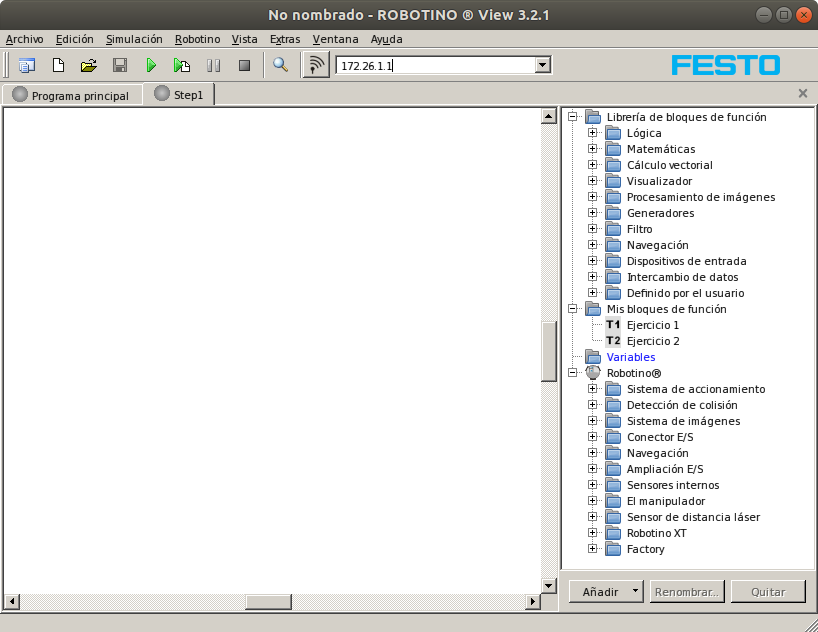
\includegraphics[width=0.9\textwidth]{images/00-inicio/01.png}
				%\caption{}
				\label{fig:inicio-01}
			\end{center}
		\end{figure}

		\column{0.6\textwidth}
		El software a utilizar en esta práctica esta desarrollado por FESTO explicitamente para trabajar con el robot móvil Robotino, con el se puede programar algoritmos simples o complejos que utilicen toda la instrumentación en el robot. Empezaremos abriendo el software Robotino View, al abrir este programa se verá una pantalla como la de la figura \ref{fig:inicio-01}. En esta ventana podemos ver del lado derecho un menu de navegación de funciones a utilizar dentro de nuestra programación.
	\end{columns}
\end{frame}

\begin{frame}
	\begin{columns}
		\column{0.6\textwidth}
		Empezaremos con un ejemplo sencillo el cual requerirá que utilicemos el motor 1 del Robotino, función que se encuentra dentro del menú Robotino, Sistema de accionamiento, Motor \# 1 como se ve en la figura \ref{fig:inicio-02}. Una vez que logremos identificar la función tan solo tenemos que arrastrarla al area central para utilizarla dentro de nuestro programa; de la misma manera encontraremos la función Corredera dentro del menú Librería de bloques de función, Dispositivos de entrada, Corredera y la colocaremos a la izquierda del motor como se ve en la figura \ref{fig:inicio-04}.

		\column{0.4\textwidth}
		\begin{figure}
			\begin{center}
				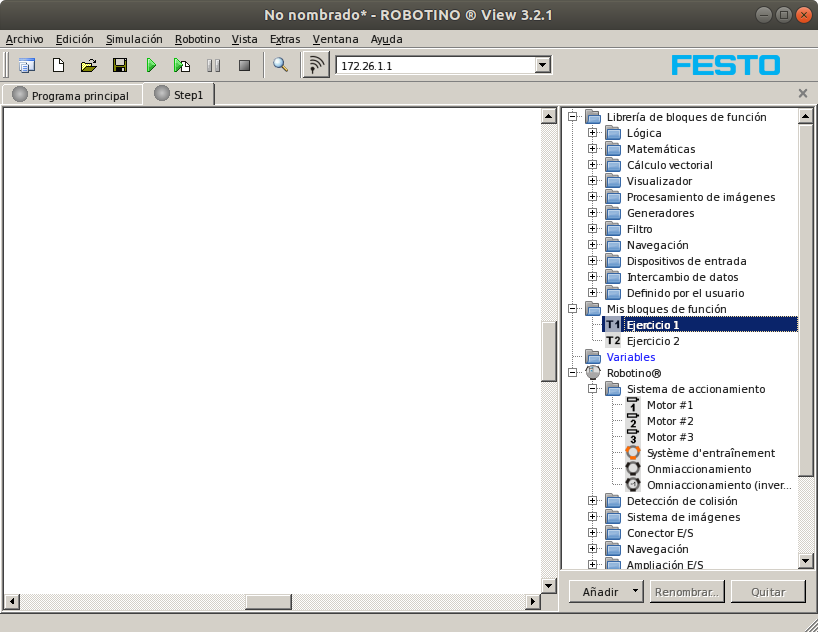
\includegraphics[width=0.9\textwidth]{images/00-inicio/02.png}
				%\caption{}
				\label{fig:inicio-02}
			\end{center}
		\end{figure}

		\begin{figure}
			\begin{center}
				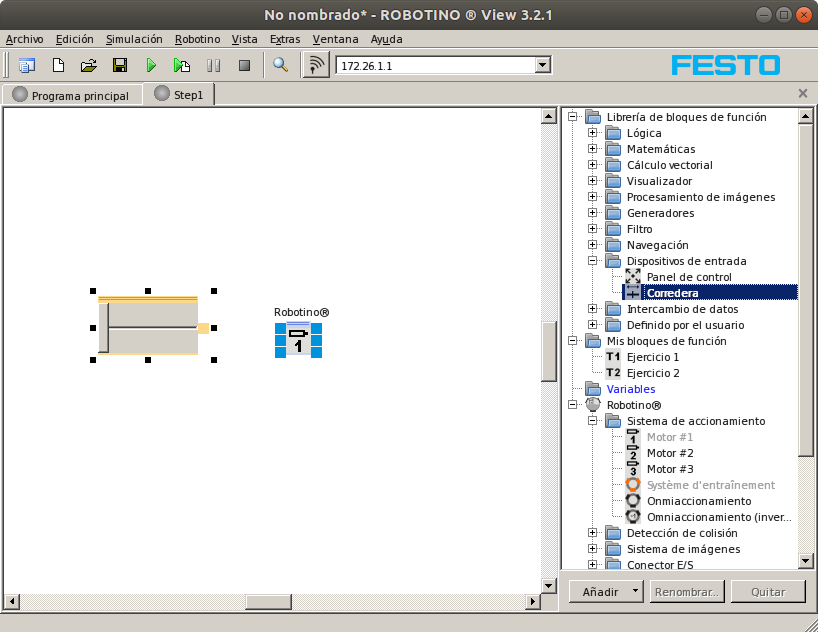
\includegraphics[width=0.9\textwidth]{images/00-inicio/04.png}
				%\caption{}
				\label{fig:inicio-04}
			\end{center}
		\end{figure}
	\end{columns}
\end{frame}

\begin{frame}
	\begin{columns}
		\column{0.4\textwidth}
		\begin{figure}
			\begin{center}
				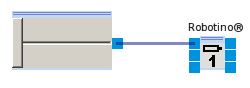
\includegraphics[width=0.9\textwidth]{images/00-inicio/05.png}
				%\caption{}
				\label{fig:inicio-05}
			\end{center}
		\end{figure}

		\column{0.6\textwidth}
		Por el momento estos elementos no tienen ninguna relación, por lo que este programa aun no haría nada, para esto necesitamos que la salida de la corredera este conectada con la entrada del motor 1, si ahora arrastras tu mouse desde el nodo de salida de la corredera al primer nodo de entrada del motor tendrás un diagrama como el de la figura \ref{fig:inicio-05}, el cual ya es un programa valido.
	\end{columns}
\end{frame}

\begin{frame}
	\frametitle{Conexión al robot virtual}
		Si intentas correr este programa con el triangulo verde ubicado en la barra de herramientas de la ventana, no pasará nada, ya que no hay ningún Robotino conectado al programa; para esto empezaremos utilizando un Robotino virtual el cual este ubicado en el software Robotino SIM, si abrimos este programa podremos ver una ventana como la de la figura \ref{fig:conexion-01}.

		\begin{figure}
			\begin{center}
				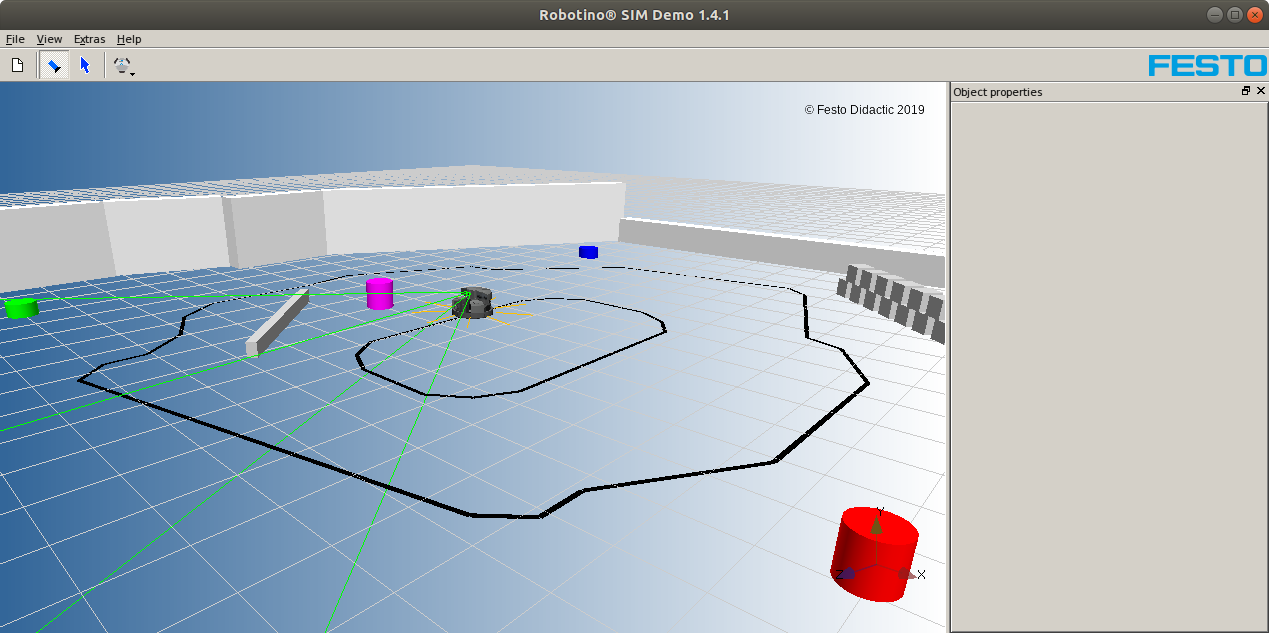
\includegraphics[width=0.8\textwidth]{images/01-conexion/01.png}
				%\caption{}
				\label{fig:conexion-01}
			\end{center}
		\end{figure}
\end{frame}

\begin{frame}
	En esta ventana podemos ver el estado del robot virtual, así como el puerto de conexion que en este caso es 8080 (dependiendo de la versión del software necesitarás estos datos) como se ve en la figura \ref{fig:conexion-03}.

	\begin{figure}
		\begin{center}
			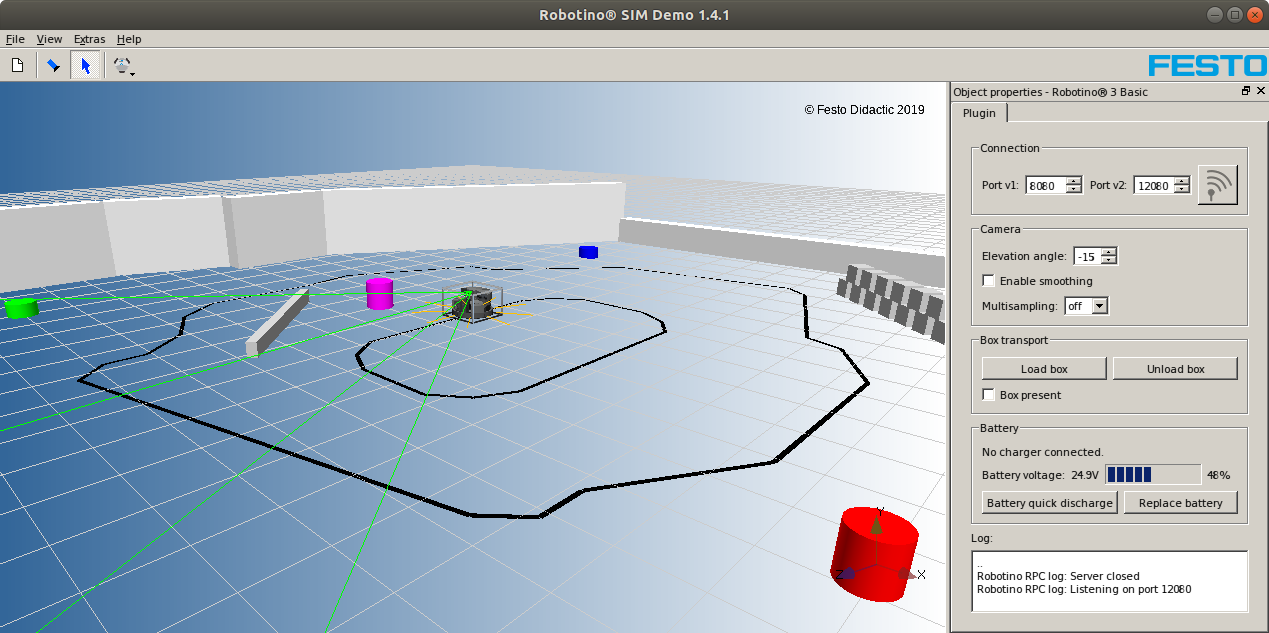
\includegraphics[width=0.8\textwidth]{images/01-conexion/03.png}
			%\caption{}
			\label{fig:conexion-03}
		\end{center}
	\end{figure}
\end{frame}

\begin{frame}
	\begin{columns}
		\column{0.6\textwidth}
		Para poder conectar nuestro ambiente de programación con el robot virtual tenemos que escribir la dirección IP en la cual el servidor del robot esta funcionando, ya que nuestro robot es virtual, esta dirección será la misma siempre 127.0.0.1, en algunas versiones del software es necesario agregar el puerto en el cual el robot esta escuchando las instrucciones, en este caso sería 127.0.0.1:8080. Si ahora damos clic sobre el icono de conexion de la izquierda tendremos el robot conectado como en la figura \ref{fig:conexion-05}

		\column{0.4\textwidth}
		\begin{figure}
			\begin{center}
				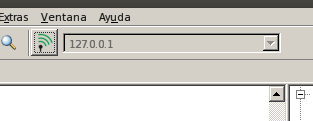
\includegraphics[width=0.9\textwidth]{images/01-conexion/06.png}
				%\caption{}
				\label{fig:conexion-05}
			\end{center}
		\end{figure}
	\end{columns}
\end{frame}

\begin{frame}
	Si ahora damos clic sobre el triangulo verde nuestro programa correrá dentro del robot virtual en tiempo real, como el de la figura \ref{fig:conexion-07}.

	\begin{figure}
		\begin{center}
			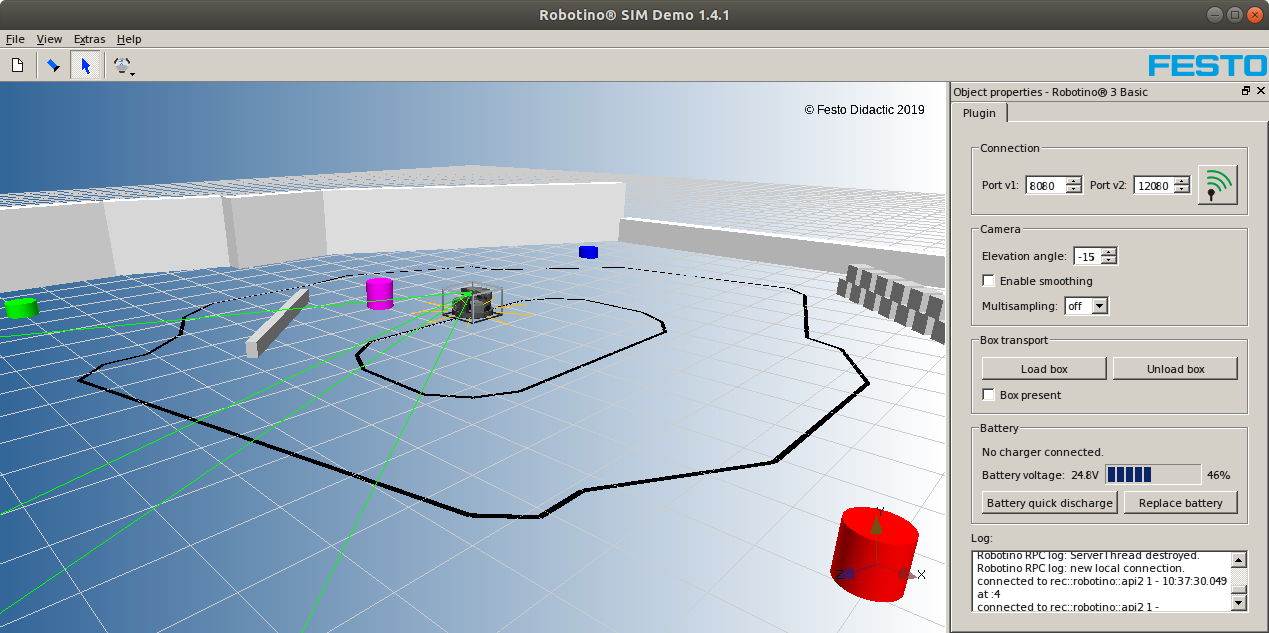
\includegraphics[width=0.9\textwidth]{images/01-conexion/07.png}
			%\caption{}
			\label{fig:conexion-07}
		\end{center}
	\end{figure}
\end{frame}

\begin{frame}
	Sin embargo nuestro robot no se mueve, no es hasta que movemos nuestra corredera como en la figura \ref{fig:pruebas-03}, que el robot empezará a moverse.

	\begin{figure}
		\begin{center}
			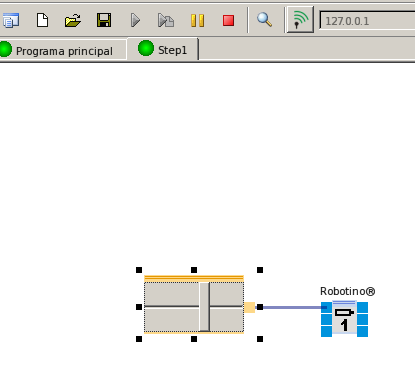
\includegraphics[width=0.5\textwidth]{images/02-pruebas/03.png}
			%\caption{}
			\label{fig:pruebas-03}
		\end{center}
	\end{figure}
\end{frame}

\begin{frame}
	\frametitle{Movimiento del robot}
	\begin{columns}
		\column{0.4\textwidth}
		\begin{figure}
			\begin{center}
				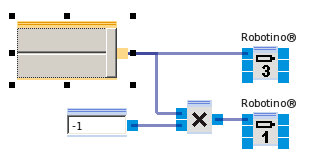
\includegraphics[width=0.9\textwidth]{images/03-movimiento/02.png}
				%\caption{}
				\label{fig:movimiento-02}
			\end{center}
		\end{figure}

		\begin{figure}
			\begin{center}
				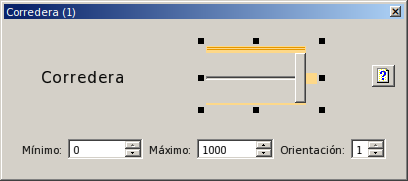
\includegraphics[width=0.8\textwidth]{images/03-movimiento/03.png}
				%\caption{}
				\label{fig:movimiento-03}
			\end{center}
		\end{figure}

		\column{0.6\textwidth}
		Por el momento nuestro robot se ve muy triste, ya que solo puede mover uno de sus motores, sin embargo esto lo podemos resolver rapidamente al hacer funcionar un motor en un sentido y otro en el contrario, con un diagrama como el de la figura \ref{fig:movimiento-02}. Si ademas modificamos el limite máximo de nuestra corredera haciendo clic secundario en la parte superior para llevarlo hasta 1000 como en la figura \ref{fig:movimiento-03}, podremos hacer mover nuestro Robotino mas agilmente.
	\end{columns}
\end{frame}

\begin{frame}
	\begin{columns}
		\column{0.6\textwidth}
		La razón por la que esto funciona para mover el Robotino hacia adelante, es que la configuración de motores del robot es como el de la figura \ref{fig:robotino-omni} en donde cada motor esta acoplado a una rueda Ilon como la de la figura \ref{fig:ilon}, la cual es capaz de moverse en cualquier dirección. Las dos ruedas traseras son las que se controlan con los motores 1 y 3, y cuando se mueven en sentidos contrarios se puede mover el robot hacia adelante o hacia atras.

		\column{0.4\textwidth}
		\begin{figure}
			\begin{center}
				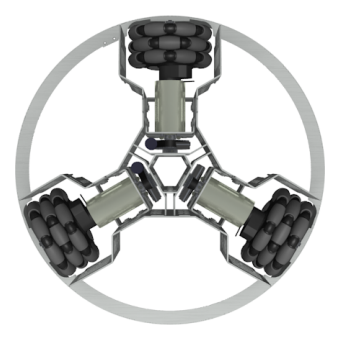
\includegraphics[width=0.8\textwidth]{images/robotino-omni.png}
				%\caption{}
				\label{fig:robotino-omni}
			\end{center}
		\end{figure}
		\begin{figure}
			\begin{center}
				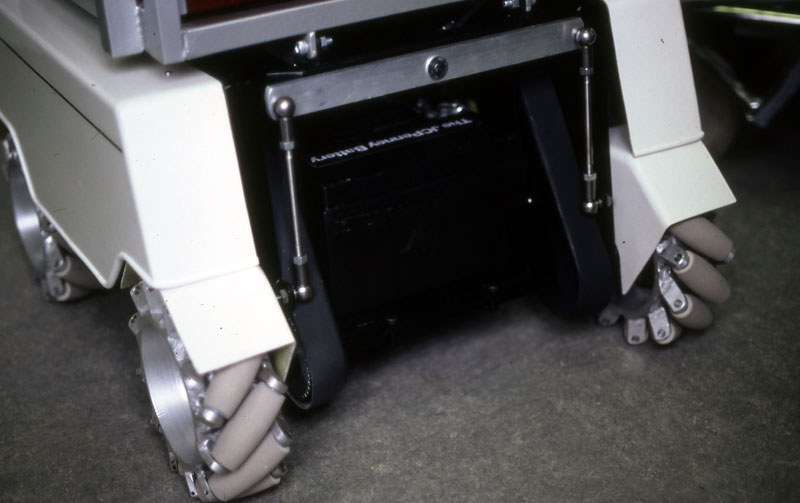
\includegraphics[width=0.8\textwidth]{images/ilon.jpg}
				%\caption{}
				\label{fig:ilon}
			\end{center}
		\end{figure}
	\end{columns}
\end{frame}

\begin{frame}
	\begin{columns}
		\column{0.5\textwidth}
		\begin{figure}
			\begin{center}
				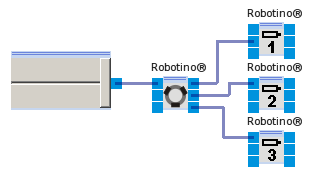
\includegraphics[width=0.9\textwidth]{images/03-movimiento/04.png}
				%\caption{}
				\label{fig:movimiento-04}
			\end{center}
		\end{figure}

		\column{0.5\textwidth}
		Sin embargo existe una función que se encarga de hacer todos los calculos necesarios para mover el Robotino de manera adecuada, si usamos el bloque Omniaccionamiento como en la figura \ref{fig:movimiento-04}, podemos obtener el mismo resultado.
	\end{columns}
\end{frame}

\begin{frame}
	\begin{columns}
		\column{0.5\textwidth}
		O bien utilizar un panel de control y mover el Robotino en todos sus ejes.

		\column{0.5\textwidth}
		\begin{figure}
			\begin{center}
				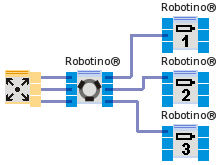
\includegraphics[width=0.9\textwidth]{images/04-omniaccionamiento/01.png}
				%\caption{}
				\label{fig:omniaccionamiento-01}
			\end{center}
		\end{figure}
		\begin{figure}
			\begin{center}
				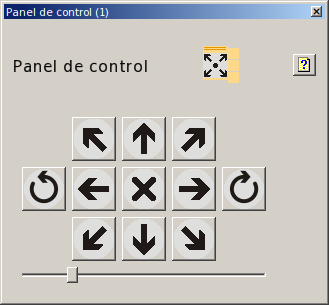
\includegraphics[width=0.9\textwidth]{images/04-omniaccionamiento/02.png}
				%\caption{}
				\label{fig:omniaccionamiento-02}
			\end{center}
		\end{figure}
	\end{columns}
\end{frame}

\begin{frame}
	\frametitle{Control}
		Si lo único que quisieramos es un carrito a control remoto, podriamos parar en este momento, sin embargo la plataforma esta diseñada para desarrollar algoritmos de control con los diferentes sensores que existen en el Robotino. Empezaremos utilizando los sensores infrarojos de distancia que se encuentran en el robotino como muestra la figura \ref{fig:sensores}.
		\begin{figure}
			\begin{center}
				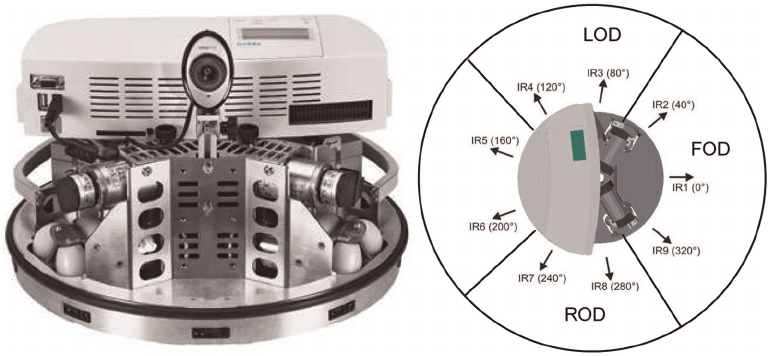
\includegraphics[width=0.8\textwidth]{images/ir-sensors.png}
				%\caption{}
				\label{fig:sensores}
			\end{center}
		\end{figure}
\end{frame}

\begin{frame}
		Para esto debemos implementar una ley de control con realimentación en lazo cerrado, es decir utilizaremos los sensores del Robotino para medir la distancia del Robotino a algún objeto y buscaremos que esta distancia disminuya hasta llegar a nuestro objetivo. El diagrama general de este sistema se verá como en la figura \ref{fig:diagrama-control}
		\begin{figure}
			\begin{center}
				\tikzstyle{block} = [draw, rectangle,
				    minimum height=3em, minimum width=6em]
				\tikzstyle{sum} = [draw, circle, node distance=1cm]
				\tikzstyle{input} = [coordinate]
				\tikzstyle{output} = [coordinate]
				\tikzstyle{pinstyle} = [pin edge={to-,thin,black}]
				\begin{tikzpicture}[auto, node distance=2cm,>=latex']
				    % We start by placing the blocks
				    \node [input, name=input] {};
				    \node [sum, right of=input] (sum) {};
				    \node [block, right of=sum] (controller) {Control};
				    \node [block, right of=controller, pin={[pinstyle]above:Perturbaciones},
				            node distance=3cm] (system) {Sistema};
				    % We draw an edge between the controller and system block to
				    % calculate the coordinate u. We need it to place the measurement block.
				    \draw [->] (controller) -- node[name=u] {$u$} (system);
				    \node [output, right of=system] (output) {};
				    \node [block, below of=u] (measurements) {Sensor};

				    % Once the nodes are placed, connecting them is easy.
				    \draw [draw,->] (input) -- node {$r$} (sum);
				    \draw [->] (sum) -- node {$e$} (controller);
				    \draw [->] (system) -- node [name=y] {$y$}(output);
				    \draw [->] (y) |- (measurements);
				    \draw [->] (measurements) -| node[pos=0.99] {$-$}
				        node [near end] {$y_m$} (sum);
				\end{tikzpicture}
				%\caption{}
				\label{fig:diagrama-control}
			\end{center}
		\end{figure}
\end{frame}

\begin{frame}
		En este caso nuestros sensores son los sensores infrarojos de distancia, estos nos darán una señal medida la cual es restada a una referencia constante, el resultado se multiplica por la ley de control, en este caso una constante con valor 100, y el resultado de esto se mete al sistema. el diagrama de control del Robotino se verá como el de la figura \ref{fig:control-01}
		\begin{figure}
			\begin{center}
				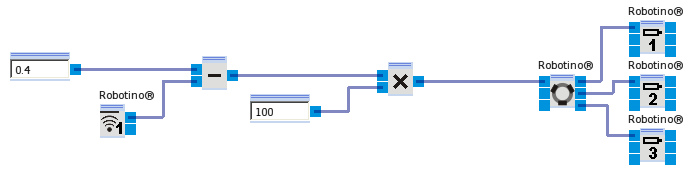
\includegraphics[width=0.95\textwidth]{images/05-control/01.png}
				%\caption{}
				\label{fig:control-01}
			\end{center}
		\end{figure}
\end{frame}

\begin{frame}
		Si queremos ver los valores de estos calculos en tiempo real, podemos encender la opción de Vista de valores en el menú Vista como en la figura \ref{fig:control-02}
		\begin{figure}
			\begin{center}
				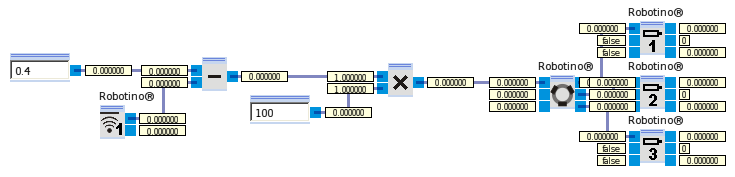
\includegraphics[width=0.95\textwidth]{images/05-control/02.png}
				%\caption{}
				\label{fig:control-02}
			\end{center}
		\end{figure}
\end{frame}

%-------------------------------------------------------------------------------
%	DESARROLLO
%-------------------------------------------------------------------------------
\begin{frame}
	\frametitle{Desarrollo}
	Diseña un algoritmo de control para el Robotino FESTO, de tal manera que el Robotino se mueva lateralmente y se pare en cuanto este a aproximadamente 30cm (el tamaño aproximado del Robotino) de la pared. Valida tu programación en simulación y corre el programa en el Robotino
\end{frame}
%-------------------------------------------------------------------------------
%	CONCLUSIONES
%-------------------------------------------------------------------------------
\begin{frame}
	\frametitle{Conclusiones}
	El alumno deberá describir sus conclusiones al final de su reporte de práctica.
\end{frame}
%-------------------------------------------------------------------------------
%	FIN DEL DOCUMENTO
%-------------------------------------------------------------------------------
\end{document}
